\documentclass{article}
\usepackage{amsmath}
\usepackage{amssymb}
\usepackage{graphicx}
\usepackage{caption}
\usepackage{subcaption}
\usepackage{float}
\usepackage{subfig}
\usepackage{hhline}
\usepackage{multirow}
\usepackage{supertabular}
\title{Homework 4}
\date{}
\author{Bastian Haase}
\begin{document}
\maketitle
\tableofcontents
\newpage 
\section{Exercise 1}
\subsection{Introduction}
In this exercise, we will calibrate a linear spring by minimizing
the difference of numerical prediction to measured data. Given a spring
who is set into motion by a displacement $u_0$ at time $t=0$, the data
provided are measurements of the distance from the equilibrium at
the time points 
\begin{align*}
  t_j=(j-1)T/(M-1) \;\; \textrm{ for } j=1,2,\ldots,M.
\end{align*}
We know from physics that the function describing the displacement
satisfies the IVP 
\begin{align}
  u''+cu'+ku=0 \textrm{ where } u(0)=u_0, u'(0)=0.
  \label{ode}
\end{align}
Here, $c$ and $k$ are two constants named the damping and spring constant
respectively. Given the data, we will try to approximate the best choice
for $c$ and $k$ such that the norm between the data provided and the
solution of the IVP is minimal. \par
This optimization problem can be stated as 
\begin{align*}
  \min_{x} f(x)
\end{align*}
where $x=(c,k)$ and 
\begin{align*}
  f(x)=\frac{1}{2}\sum_{j=1}^{M}\left ( u(t_j;x)-u_j \right )^2.
\end{align*}
Here, $u_j$ denotes the data point measured at time $t_j$. We can see that this
problem is a least squares problem.
\subsection{The Objective Function and its Gradient}
In this section, we will use the notation used in class for
least squares problems. Hence, we can write 
\begin{align*}
f(x)=\frac{1}{2}\sum_{j=1}^M r_j(x)^2
\end{align*}
where 
\begin{align*}
  r_j(x)= u(t_j;x)-u_j.
\end{align*}
In order to determine the gradient of $f$, we need $\frac{\partial u}{\partial c}$
as well as $\frac{\partial u}{\partial k}$. In view of (\ref{ode}), one can compute that
 $\frac{\partial u}{\partial c}$ is the unique  solution of the IVP 
\begin{align}
   y''+cy'+ky+u'=0 \textrm{ where } y(0)=0, y'(0)=0,
\label{odec}
\end{align}
whereas  $\frac{\partial u}{\partial k}$ is the solution of
\begin{align}
   y''+cy'+ky+u=0 \textrm{ where } y(0)=0, y'(0)=0.
\label{odek}
\end{align}
The derivation of these two formulas was discussed in class by use of an ad-hoc method. One can also argue by
means of the definition of the derivative to show that the partial derivatives satisfy the given ODEs. Interpreting $u$ as a function of $t,c$ and $k$ and
using the symmetry of mixed partial derivatives, one readily sees  that 
\begin{align*}
 &\left( \frac{\partial u}{\partial c}\right)''+\left(c \left(\frac{\partial u}{\partial c}\right)'+u' \right)+k \frac{\partial u}{\partial c} \\
= & \frac{\partial}{\partial c}\left(u''+cu'+ku  \right)=\frac{\partial}{\partial c} 0 =0
\end{align*}
 The boundary conditions can be derived using Lagrangians or the definition of the derivative. Note that the derivation for $k$ is analogous. \par
In practice, we will have to solve these ODEs for various values of $c$ and $k$. These ODEs could potentially be stiff and we will therefore solve them with the
solver \emph{ode23s}. \par
For fixed $(c,k)$ we need to be able to evaluate the functions
$u$, $\frac{\partial u}{\partial c}$ and $\frac{\partial u}{\partial k}$
at the points $t_j$. As our solver uses a dynamic grid dependent on the
given equation, we will specify that these points are among the ones computed. However,
to solve the IVPs \ref{odec} and \ref{odek}, we need to be able to evaluate $u$ at any point $t \in [0,T]$. To overcome this issue,
we will interpolate the return of ode23s linearly. The error of this interpolation
is quadratic in terms of the step size, as is well known by the theory of Lagrange-interpolation. \par
Once we have obtained the partial derivatives of $u$, we can compute the gradient of $f$
via 
\begin{align*}
  J(x)_{i,j}&=\frac{\partial r_i}{\partial x_j} \\
  \nabla f(x)&=J(x)^{T} r(x) \\
  \nabla^2 f(x)& =J(x)J(x)^T+\sum_{j=1}^M r_j(x) \nabla^2 r_j(x).
\end{align*}
Note that that the computation of the first summand of the Hessian is relatively
cheap when one needs to compute the gradient anyway. Subsequently, we will
use the term 
\begin{align*}
 H= J(x)J(x)^T
\end{align*}
as an approximation of our Hessian. When we speak of the approximated Hessian,
we will always address this specific term throughout this document.\par
In figure \ref{taylor}, we can see that our gradient gives us quadratic convergence up to a distance of roughly $10^{-4}$, then
the error is linear. This can be explained by the fact that we introduce more sources of errors by use of linear interpolation
and ODE solvers. These errors become dominant for small distances and therefore overshadow the usual quadratic convergence of 
the first order Taylor polynomial.
\begin{figure}
    \centering
        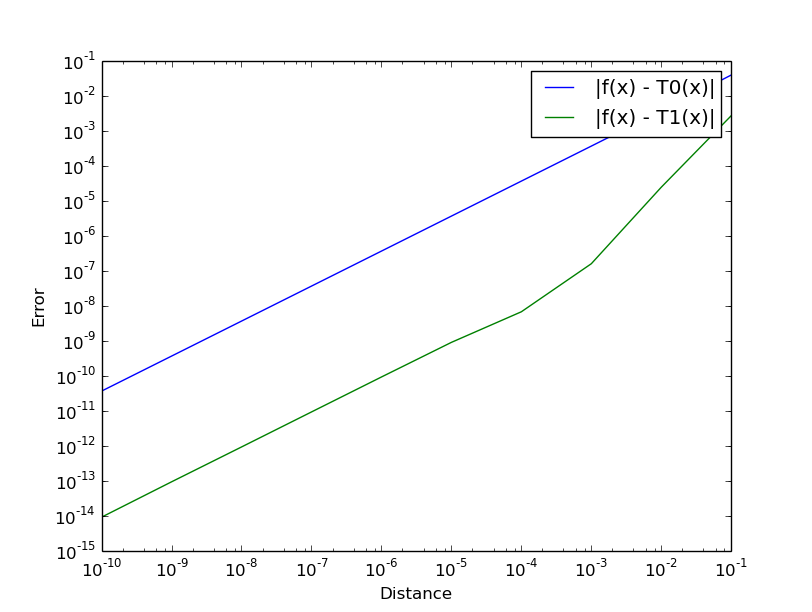
\includegraphics[width=0.65\textwidth]{check_derivative}
        \caption{Error of Taylor Polynomials of degree 0 and 1}
        \label{taylor}
\end{figure}
\subsection{Convergence on $[0.1,5]^2$}
In this section, we will analyze the convergence of the Gauss-Newton method
applied to our objective function $f$ on an equidistant $20 \times 20$ grid
of $\Omega=[0.1,5]^2$.
\subsubsection{The Setup}
We will use the Gauss-Newton method for our approximation. In our code,
this was realized by replacing the Hessian by our approximation in the
method NewtonCG of the OptimTools package. By taking a closer look at the code,
this is equivalent to using damped Newton with this approximation.\par
We also use standard armijo-line search with a starting step length of 1. We iterate until the 
maximum number of iterations (=100) is reached or our current iterate is accurate within
a tolerance of $10^{-2}$. On this grid, the maximum number of iterations was never reached. Figure \ref{contour} displays a contour plot of $\log(f)$ to give us
an idea of what we should expect when applying Gauss-Newton and BFGS. As the logarithm is
monotonically increasing, $\log(f)$ attains its minimum at the same point and has the same contour
lines as $f$.
\begin{figure}
    \centering
        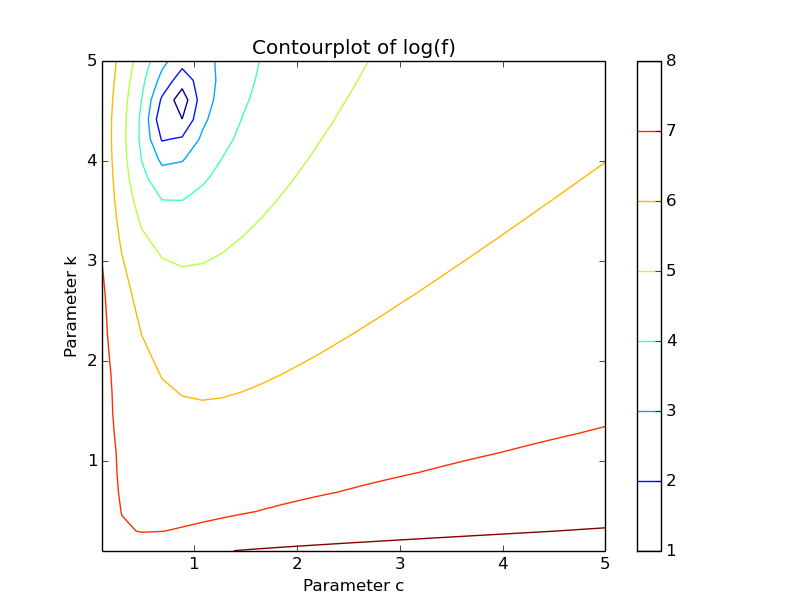
\includegraphics[width=0.65\textwidth]{contour}
        \caption{Contour plot of $\log(f)$}
        \label{contour}
\end{figure}
As we can see from this plot, the minimum of the objective function is approximately attained at $(0.8,4.5)$.
Based on the contour lines and the curvature, Gauss-Newton should perform much better for $k>c$
than for $k<c$ as the much higher residuals for $k<c$ suggest.
\subsubsection{Interpretation}
We will display the run time, the number of iterations and the convergence at 
every point of the grid in figure \ref{global}. Note that this matrix plot corresponds
to the region $\Omega$ and the $x$ and $y$-axis correspond to $c$ and $k$ respectively.
Let us first look at plot (a), which displays whether we reached a tolerance of $10^{-2}$. Here, white represents convergence and black represents failure of the method. As the contour plot suggested,
we get convergence at every point  where $c>k$. However, for $c<k$ there are many points where our
method fails. The cause for failure at \textbf{all} of these points was that the ODE solver could
not solve the IVP within the given accuracy, which was $10^{-8}$. This problem could not be resolved by modifying the accuracy. It seems to be the case that the differential equations become too stiff for large residuals. \par
\begin{figure}
    \centering
    \begin{subfigure}[b]{0.45\textwidth}
        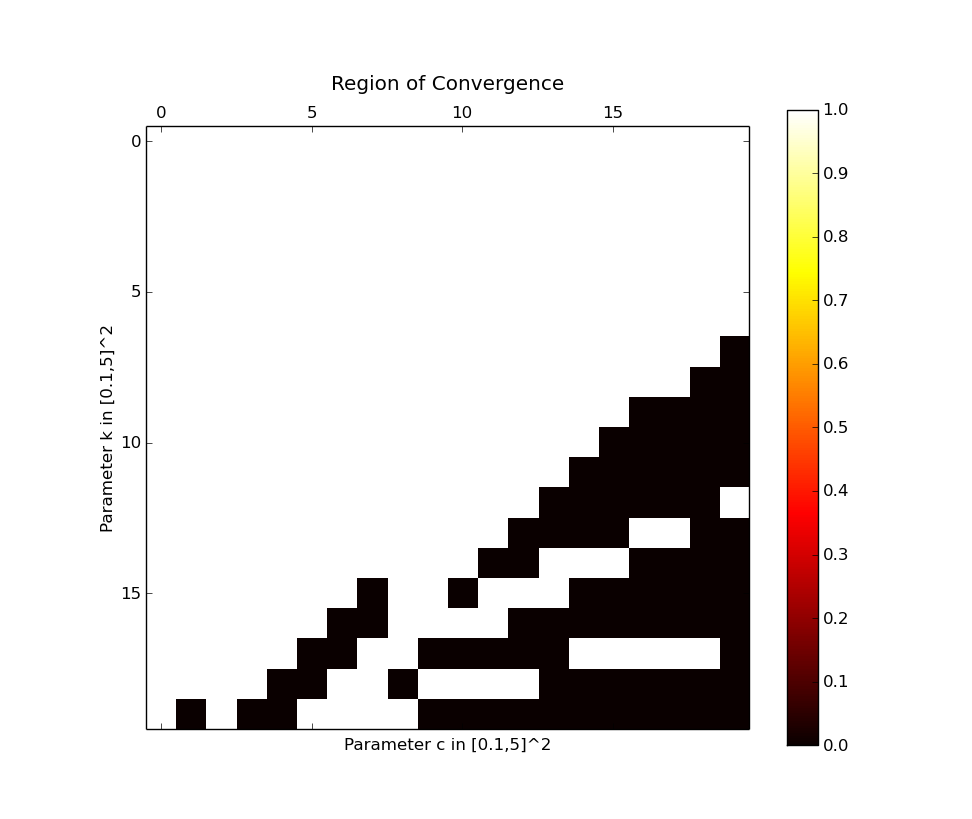
\includegraphics[width=\textwidth]{global_conv}
        \caption{Region of Convergence}
        \label{fig:re}
    \end{subfigure}
    \begin{subfigure}[b]{0.45\textwidth}
        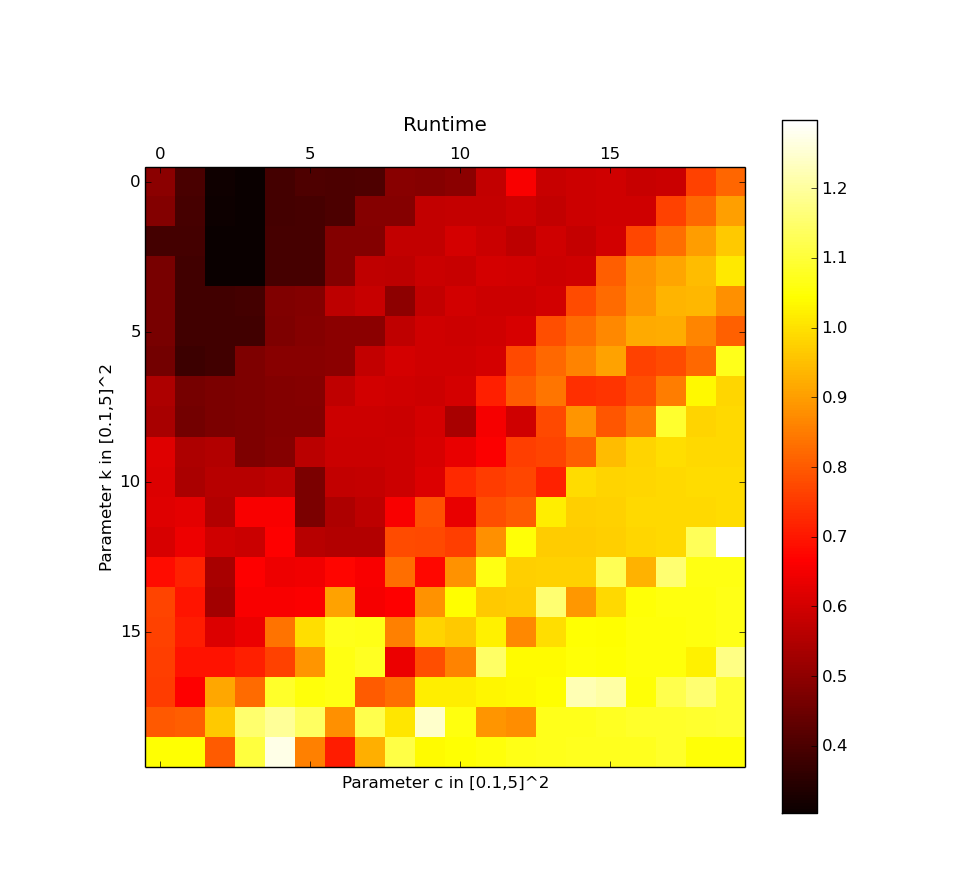
\includegraphics[width=\textwidth]{global_run}
        \caption{Runtime}
        \label{fig:ru}
    \end{subfigure}
    \begin{subfigure}[b]{0.45\textwidth}
        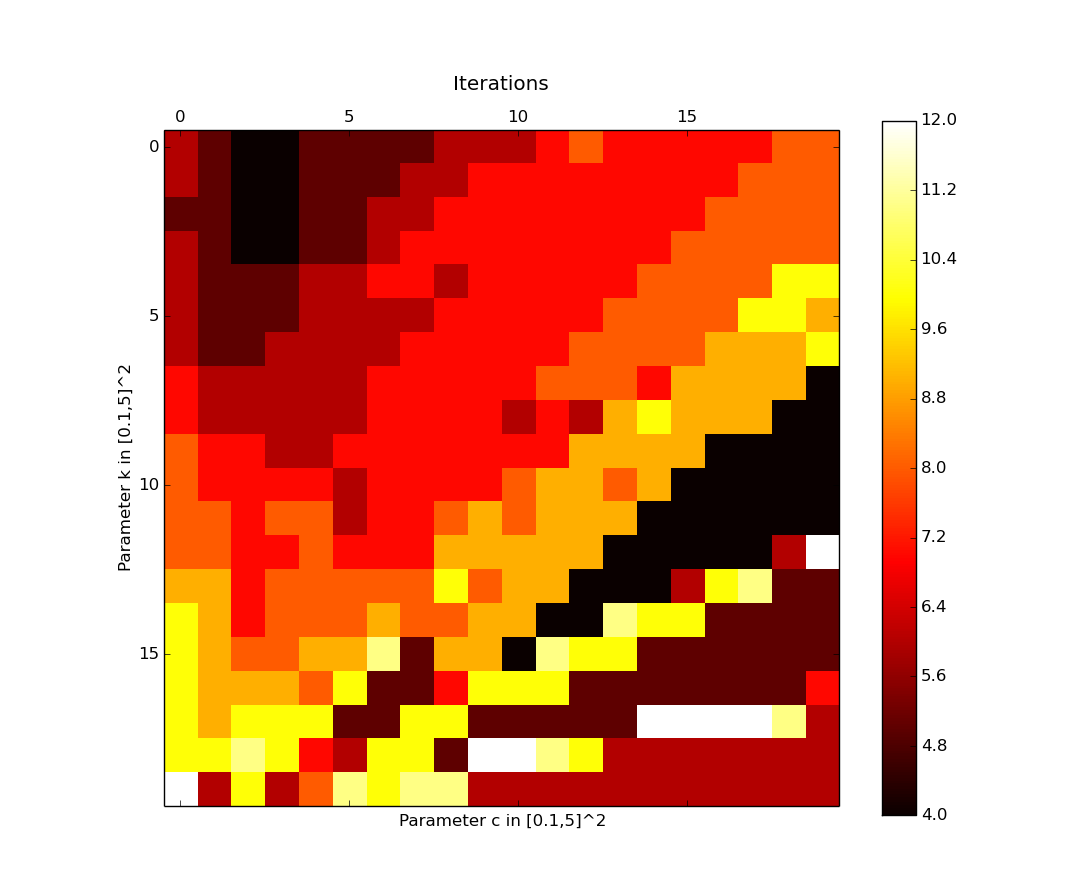
\includegraphics[width=\textwidth]{global_iter}
        \caption{Iterations}
        \label{fig:it}
    \end{subfigure}
    \caption{Global Convergence}
    \label{global}
\end{figure}
When we look at the run time, it is interesting to see that the contour plot did not mislead us.
The convergence is much faster for values $c<k$, which is on par with our expectation.
Apart from that the run time decreases as we get close to our estimation of the parameters,
which reaffirms our guess. \par
Lastly, the number of iterations looks at first glance a little chaotic. However, note that
for $c>k$, the area where the number of iterations is low corresponds to the points where the method failed. I guess it is desirable for a method to fail quickly if it fails, this should however not
distract from the fact that for converging starting points the number of iterations is lower when
$c<k$, which agrees with the run time results. Hence, we can again conclude that the best guess for
the parameter is $(0.8,4.5)$. 
\subsection{Gauss-Newton vs BFGS}
In this section, we will compare the Gauss-Newton method to a standard implementation of
BFGS. The setting is the same as last time, but we will restrict ourselves to
the starting point $(1,1)$. We have measured the run time, the number of iterations and the
number of IVPs that had to be solved.
\begin{table}[H]
  \centering
  \begin{tabular}{|l|c|c|c|c|c|}
    \hline
   \textbf{Method} & \textbf{Iterations} & \textbf{Run time} &\textbf{Memory} &\textbf{Eval. f,df,H} & \textbf{IVPs} \\ \hline
  BFGS &26 &1.628233&14.3Mb &76,27,0& 130 \\ \hline
  Gauss-Newton &8 &0.617532&5.6Mb &18,8,8& 50 \\ \hline
  \end{tabular}
  \caption{Performance Comparison $x_{0}=(1,1)$, Run time in sec}
  \label{tab:perform}
\end{table}
Even though the problem is very different, these results are similar to the ones obtained
in the last homework problem. Even though we use a different way to approximate our Hessian,
it turns out that the a Newton method with approximated Hessian often performs better than
a standard BFGS. Gauss-Newton needs less iterations, has a faster run time and less function
and gradient evaluations. Even though BFGS avoids the evaluation of the Hessian, this does not
have a huge impact as evaluating our approximation of the Hessian requires the same ODEs to be solvend and replaces a matrix-vector product by a matrix-matrix product. So, while it costs more,
the effect in this particular problem is not very strong. Also, the number of IVPs that need to be solved is lower for Gauss-Newton
which is probably the main reason for the quicker run time. We can also observe that the memory consumption of BFGS is much higher, although this difference might be greatly reduced by a limited-memory implementation of BFGS.\par
In figure \ref{iterates}, you can see the iterates of both Gauss-Newton and BFGS.
\begin{figure}
    \centering
    \begin{subfigure}[b]{0.45\textwidth}
        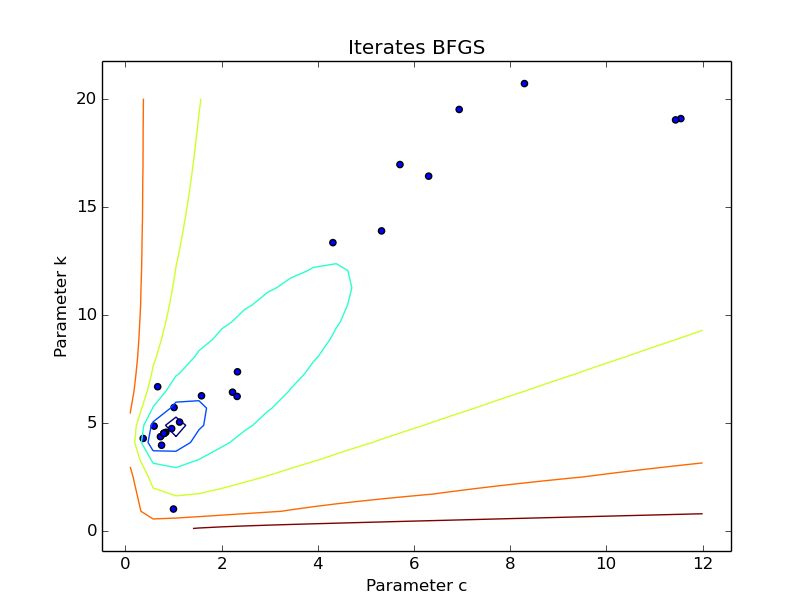
\includegraphics[width=\textwidth]{scatter_bfgs}
        \caption{BFGS Iterates}
        \label{fig:g}
    \end{subfigure}
    \begin{subfigure}[b]{0.45\textwidth}
        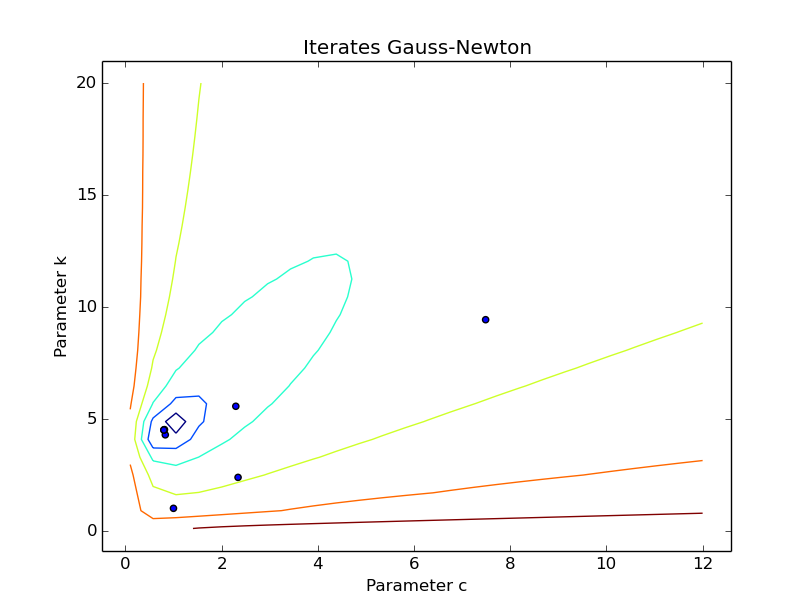
\includegraphics[width=\textwidth]{scatter_gauss}
        \caption{Gauss-Newton Iterates}
        \label{fig:t}
    \end{subfigure}
    \caption{Iterates on Contour Plot of $\log(f)$}\label{fig:animals}
\label{iterates}
\end{figure}
It is interesting to note that the iterates of both methods look almost chaotic.
As both of them use approximated curvature information, it is not surprising that one
can not predict the next iterate based on the contours and the position of the solution. However,
it might surprise that especially some of the iterates of BFGS are far out and are much further away from the solution than our initial guess in the euclidean norm. But, we already observed the
big difference in performance between the cases $c<k$ and $c>k$. Here, our initial case
satisfies $c=k$ and is therefore just on the edge. Comparing both methods, we can observe yet again that Gauss-Newton performs superior. \par
 In figure \ref{his}, the norm of $f(x_k)$ and $\nabla f(x_k)$ are visualized for BFGS and Gauss-Newton.
\begin{figure}
    \centering
    \begin{subfigure}[b]{0.45\textwidth}
        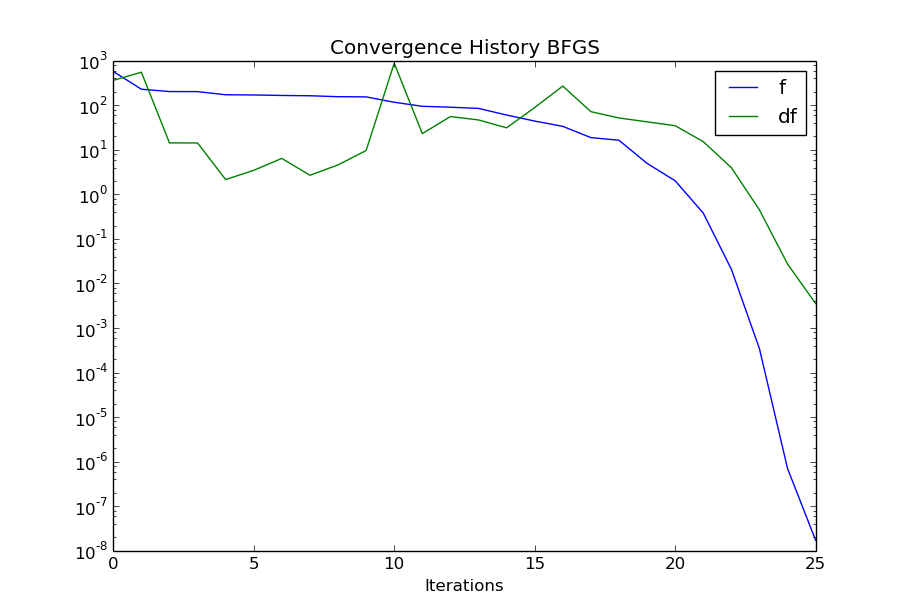
\includegraphics[width=\textwidth]{conv_his_bfgs}
        \caption{BFGS}
       
    \end{subfigure}
    \begin{subfigure}[b]{0.45\textwidth}
        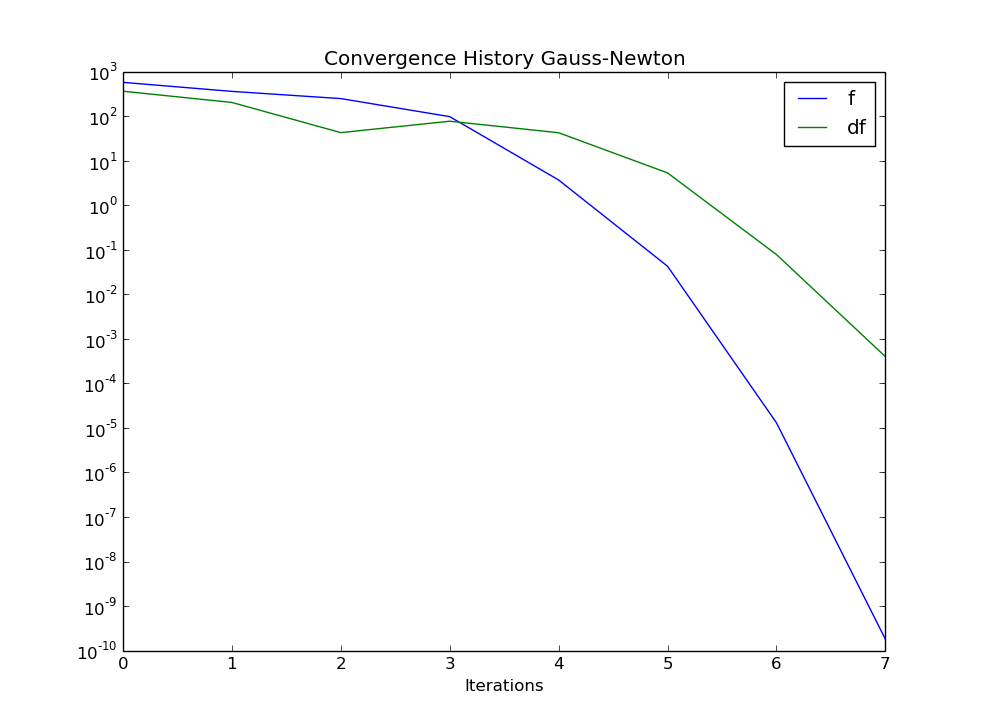
\includegraphics[width=\textwidth]{conv_his_gauss}
        \caption{Gauss Newton}
       
    \end{subfigure}
    \caption{Convergence History}\label{his}
\end{figure} 
The first noteworthy observation is that the norm of the gradient does not decrease monotonically
in both cases. This was not to be expected, as there is no general result on monotonically
decreasing gradients for any of the methods. When we look at the norm of the objective function,
we can see that the convergence starts off very slowly and then dramatically increases at the end.
Thus, our convergence is much better when we are close to the solution. This is not surprising
for any Newton or quasi-Newton method. In this case, the fact that the residuals are much smaller
close to the solution, is one of the reasons why Gauss-Newton performs so much better close to the solution. We can conclude that for least squares problems where the optimal solution has small residuals, the choice of a good initial guess can be key.
\subsection{Noise}
In this section we will compare BFGS and Gauss-Newton at the point $(1,5)$.
Additionally, we have added noise to the data and we will analyze how the noise
affects our result. The noise is generated by use of \emph{randn} and $\epsilon$ will
denote the maximum norm of our noise. The following table shows how the noise affects the
computational costs.
\begin{table}[H]
  \centering
  \begin{tabular}{|l|c|c|c|c|}
    \hline
   \textbf{Method} & \textbf{Iterations} & \textbf{Run time}&\textbf{Eval. f,df,H} &\textbf{IVPs} \\ \hline \hline
  BFGS, $\epsilon=0$ &7 &0.61078 &28,8,0&44 \\ \hline
  Gauss-Newton, $\epsilon=0$ &5 &0.3541 &9,5,5&29 \\ \hline \hline
  BFGS, $\epsilon=10^{-8}$ &7 &0.61121 &28,8,0&44 \\ \hline
  Gauss-Newton, $\epsilon=10^{-8}$&5 &0.3569 &9,5,5 &29 \\ \hline \hline
 BFGS, $\epsilon=1$ &7 &0.789382 &27,8,0&43 \\ \hline
  Gauss-Newton, $\epsilon=1$ &5 &0.547566 &9,5,5&29 \\ \hline \hline
 BFGS, $\epsilon=10$ &9 &9.589382 &32,10,0&52 \\ \hline
  Gauss-Newton, $\epsilon=10$ &8 &4.547566 &16,8,8&48 \\ \hline 
  \end{tabular}
  \caption{Performance Comparison with Noise $x_{0}=(1,5)$, Runtime in sec}
  \label{tab:perform}
\end{table}
Note that the performance depends on the random numbers, not just their norm. Hence, the results
in this table should not be understood absolute, but relative with respect to the random
numbers.  \par
We can see from this table that both methods are relatively robust when it comes to noise.
For $\epsilon\leq 1$, the performance is not significantly influenced. When we set $\epsilon=10$,
which is an unreasonable large noise given that the maximum displacement of our spring is also 10,
we can see that the methods converge slower but not as much as one might expect.\par
When I really tried to break things, I found out that BFGS performs much worse than Gauss-Newton
for $\epsilon=100$ and both mehtods failed to converge for $\epsilon=1000$. But, such a noise
makes results worthless anyway, so these results should not be considered when comparing the 
robustness and efficiency of both algorithms.\par
From the data obtained, it is hard to say which method is more robust. Both methods scale similarly
with the amount of noise and in this setting one can say that they both handle a reasonable amount
of noise very well.\par
We will now take a closer look at the accuracy of our approximation by
plotting our final displacement in figure \ref{fig:animals}  side-by-side with the actual solution and
the noised data.
\begin{figure}
    \centering
    \begin{subfigure}[b]{0.45\textwidth}
        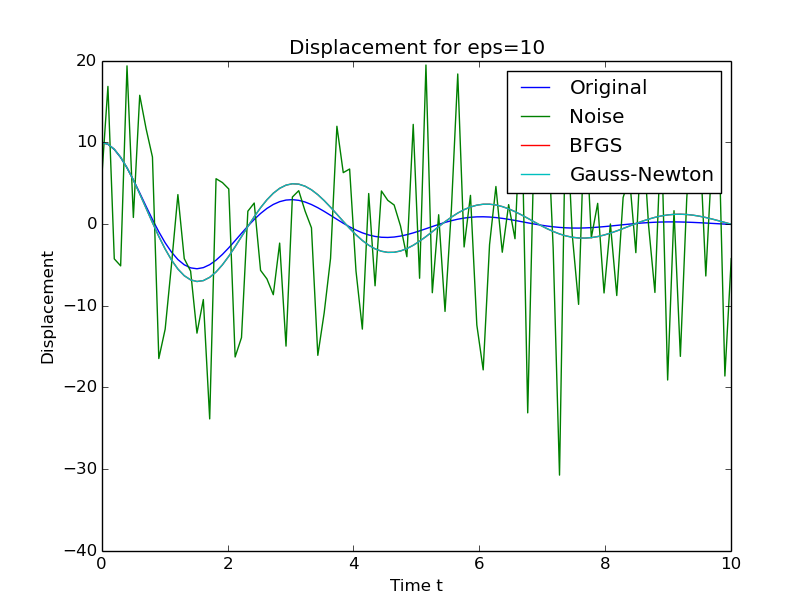
\includegraphics[width=\textwidth]{noise0}
        \caption{$\epsilon=10$}
        \label{fig:gull}
    \end{subfigure}
    \begin{subfigure}[b]{0.45\textwidth}
        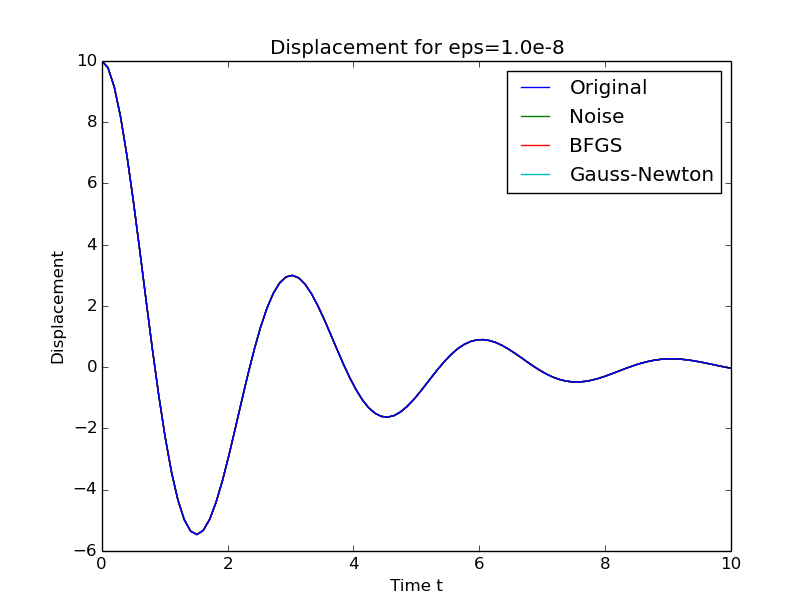
\includegraphics[width=\textwidth]{noise8}
        \caption{$\epsilon=10^{-8}$}
        \label{fig:tiger}
    \end{subfigure}
    \begin{subfigure}[b]{0.45\textwidth}
        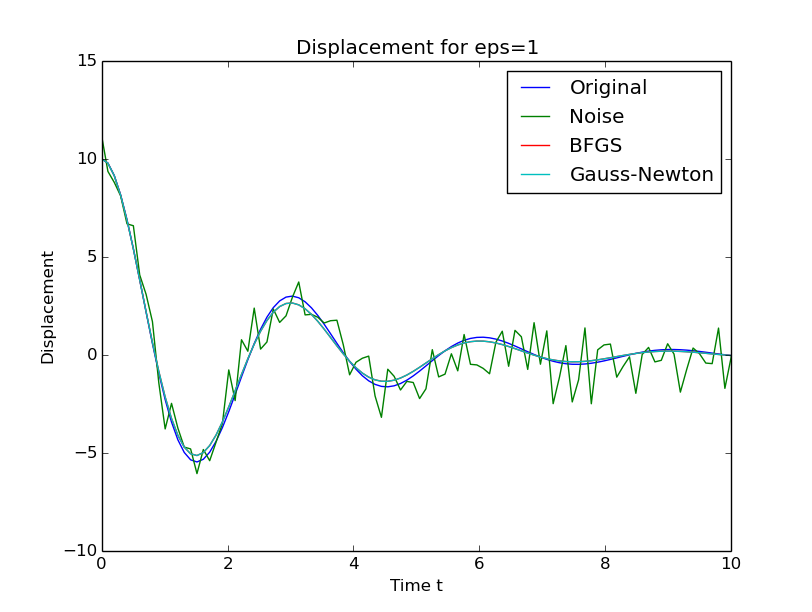
\includegraphics[width=\textwidth]{noise1}
        \caption{$\epsilon=10^{-2}$}
        \label{fig:mouse}
    \end{subfigure}
    \caption{Plots of displacement for various $\epsilon$}\label{fig:animals}
\end{figure}
We can see that the approximated solutions are always very close provided that the methods
converge. Even when the noise is very strong, the approximated parameters are further off, but the displacement is still surprisingly close. From these pictures, it seems plausible
that a noise of $10^{-8}$ might be negligable in most circumstances.
Both methods always converge to the same solution, so the only difference in noise handling lies in computational costs.\par
 Based on this one could hypothesize that for similar types of problems small
noise is negligible both in computational costs and acccuracy of approximation.
\end{document}


\begin{figure}[H]
  \centerline{
  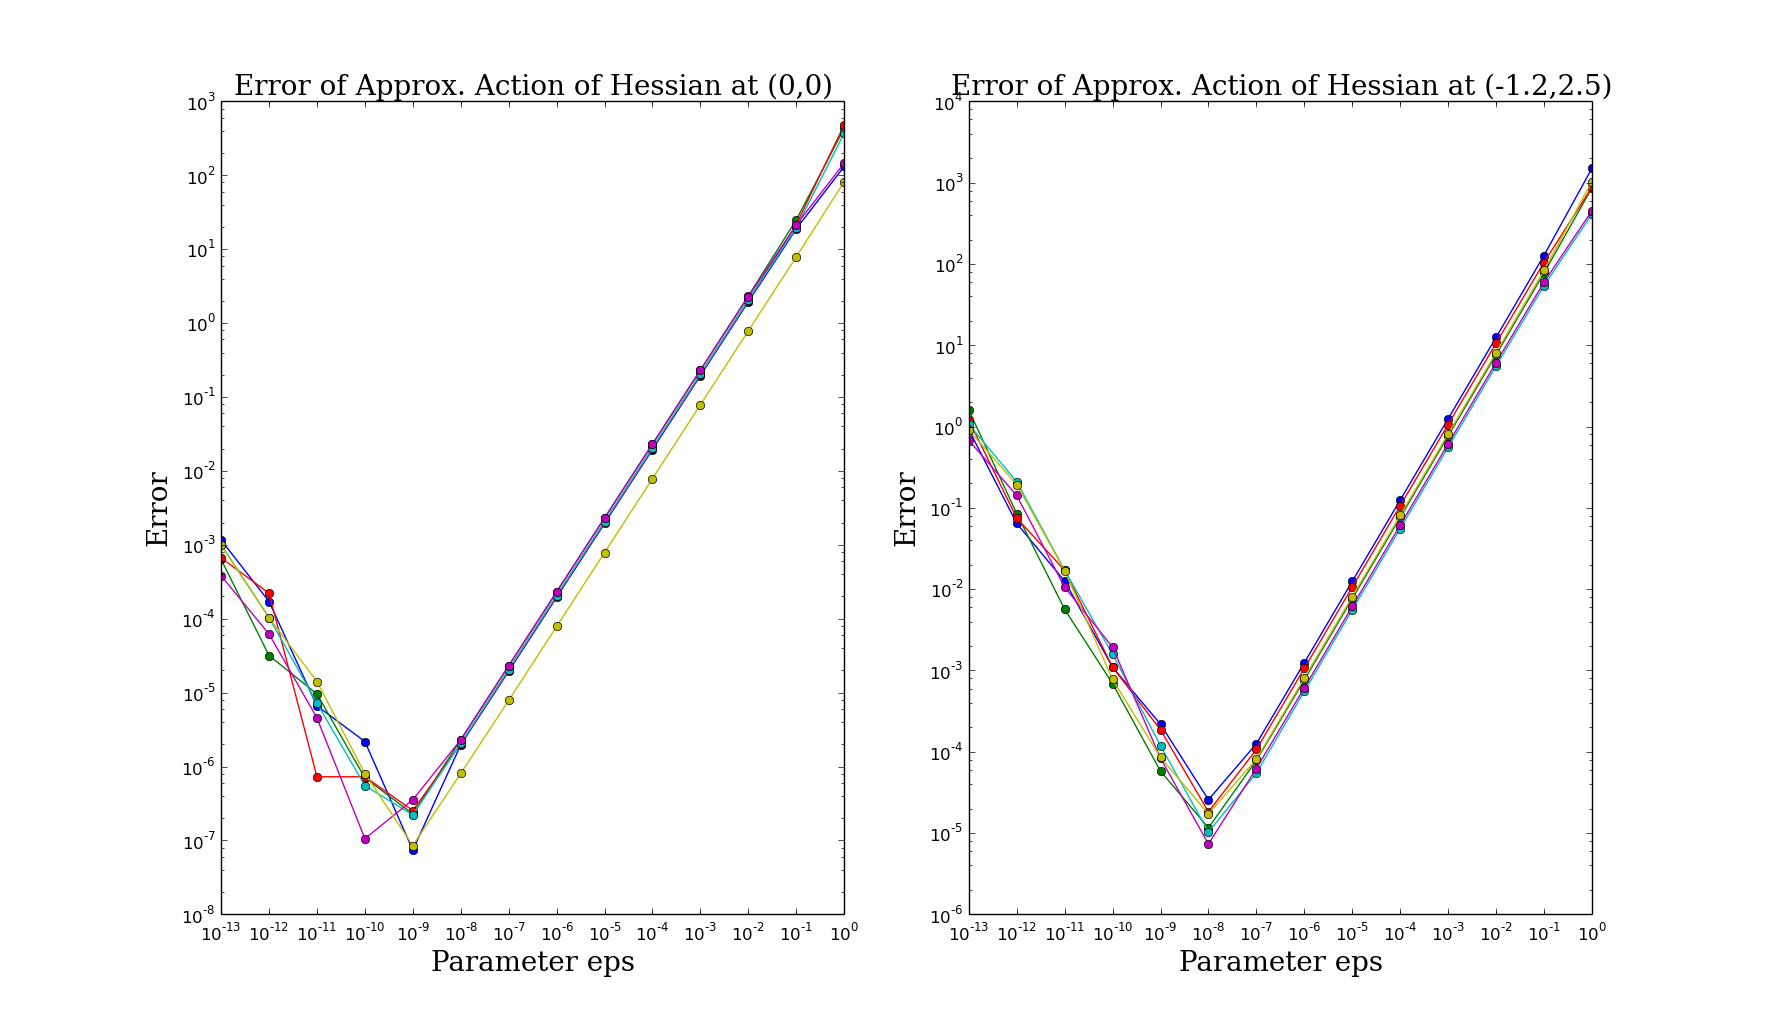
\includegraphics[scale=0.3]{action.png}
  }
  \caption{Error of Approximating Hessian}
\label{action}
\end{figure}


